\documentclass{article}

% Language setting
% Replace `english' with e.g. `spanish' to change the document language
\usepackage[english]{babel}

% Set page size and margins
% Replace `letterpaper' with `a4paper' for UK/EU standard size
\usepackage[letterpaper,top=2cm,bottom=2cm,left=3cm,right=3cm,marginparwidth=1.75cm]{geometry}

% Useful packages
\usepackage{amsmath}
\usepackage{amssymb}
\usepackage{graphicx}
\usepackage[colorlinks=true, allcolors=blue]{hyperref}

\usepackage{indentfirst} % Indent first paragraph after section

\title{Graphs and Networks in Artificial Intelligence}
\author{Denys Mykhailov}

\begin{document}
\maketitle

\begin{abstract}

      This essay explores the intersection of graph theory and artificial intelligence, focusing on the development and application of Graph Neural Networks (GNNs).
      It traces the historical roots of graph-based AI, discusses key theoretical foundations, and highlights major developments such as Graph Convolutional Networks (GCNs) and Graph Attention Networks (GATs).
      The essay also examines current applications of GNNs in various domains, influential contributors to the field, and open challenges for future research.
      By understanding the evolution and capabilities of GNNs, we gain insights into how these models can effectively learn from graph-structured data, enabling advancements in AI systems that leverage relational information.

\end{abstract}

\section{Introduction}

Graphs are mathematical structures used to model pairwise relations between entities.
A graph consists of \textbf{nodes} (vertices) representing entities and \textbf{edges} representing connections or relationships between these entities.
Due to their flexibility in representing complex systems, graphs appear in countless real-world scenarios – from social networks linking people, to molecules with atoms connected by chemical bonds, to knowledge graphs encoding facts.
In the field of Artificial Intelligence (AI), graphs have long been used as a natural way to represent knowledge and structure (for example, \textbf{semantic networks} in early AI represented knowledge as nodes and links).
However, only recently have we developed powerful learning algorithms, called \textbf{Graph Neural Networks (GNNs)}, that can directly learn from graph-structured data rather than just using graphs as static data structures.
These GNNs extend classical neural networks to work on arbitrary graphs, enabling AI systems to better exploit \textbf{relational information}.

The rise of GNNs represents a convergence of graph theory (a branch of discrete mathematics dating back to the 18th century) and modern deep learning.
In this essay, we explore the origins of this interdisciplinary field, its key theoretical foundations and results, major developments (such as GCNs and GANs), current applications of graph-based AI, influential contributors, and open challenges for the future.

\subsection{Origins of Graph Theory and Early Graph Applications in AI}

\textbf{Graph theory} as a mathematical field originated from the famous Königsberg bridge problem solved by Leonhard Euler in 1736 \cite{carlson2019konigsberg}.
Euler’s solution – proving that no path exists that crosses each of the city’s seven bridges exactly once – is regarded as the first theorem in graph theory and marked the birth of graph theory as a discipline.
Over the next two centuries, graph theory was developed by many mathematicians, including Cayley, Kirchhoff, and Whitney, who established foundational concepts such as connectivity, planarity, and graph coloring.

% photo of Königsberg bridges
\begin{figure}[h]
      \centering
      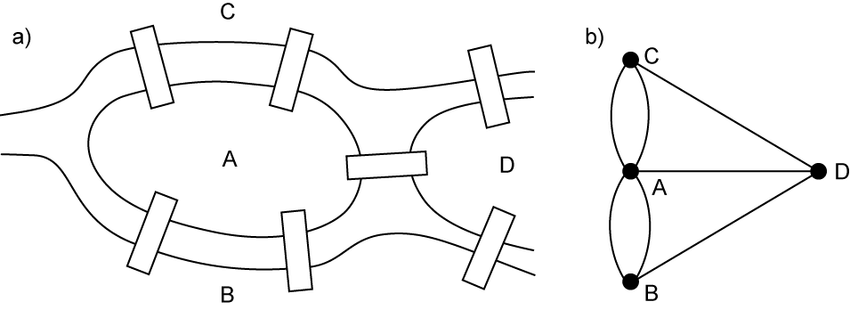
\includegraphics[width=0.4\textwidth]{../assets/konigsberg-bridges.png}
      \caption{The original seven bridges of Königsberg, which inspired Euler's work on graph theory.}
      \label{fig:konigsberg-bridges}
\end{figure}

\subsection{Early Graph Applications in AI}

In the early days of AI, graphs were primarily used to represent knowledge, relationships and reasoning.
Early AI pioneers like Marvin Minsky and others introduced \textbf{semantic networks} (graph-based knowledge representations) in the 1960s and 1970s to encode relationships between concepts in natural language understanding \cite{kelemen2007neural}.

Around the same time, probabilistic graphical models were developed – \textbf{Bayesian networks} introduced by Judea Pearl in the 1980s \cite{pearl1995bayesian} and \textbf{Markov random fields} \cite{lang2024abstract} – which leveraged graph structures (directed or undirected graphs) to represent probabilistic dependencies among variables for AI reasoning using joint \textbf{probability distributions} and \textbf{factor graphs} \cite{loeliger2004factor}.

These early uses of graphs in AI, however, treated graphs as static structures or as a backdrop for algorithms; there was \textit{no concept} of learning on graphs with neural networks yet.

% photo of  Bayesian networks and Markov random fields
\begin{figure}[h]
      \centering
      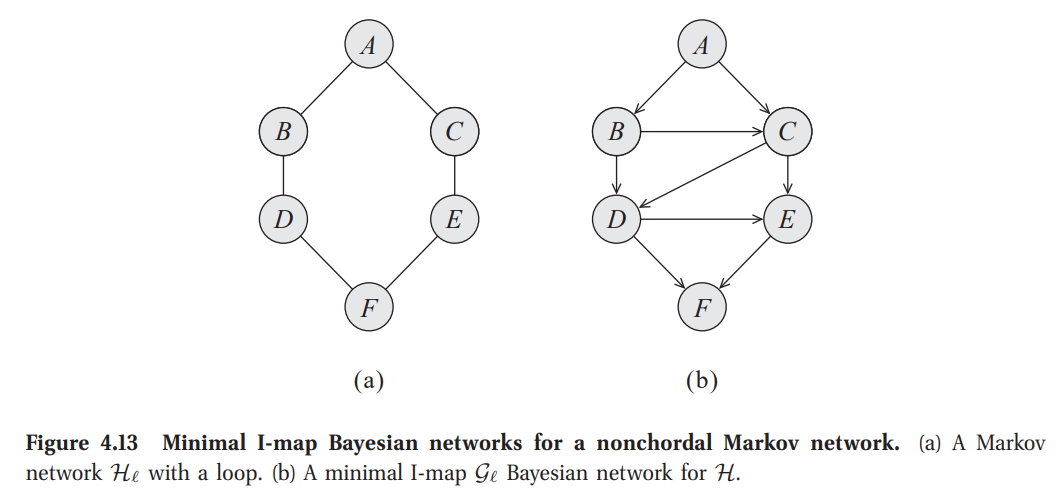
\includegraphics[width=1\textwidth,trim=0 100 0 0,clip]{../assets/bayesian-and-markov-networks.png}
      \caption{\textbf{Minimal I-map Bayesian networks for a nonchordal Markov network.} \\ (a) A Markov network $\mathcal{H}_\ell$ with a loop. (b) A minimal I-map $\mathcal{G}_\ell$ Bayesian network for $\mathcal{H}_\ell$.}
      \label{fig:bayesian-networks}
\end{figure}


\bibliographystyle{plain}
\bibliography{references}

\end{document}
